\documentclass[reqno,12pt,oneside]{report}
\usepackage[utf8]{inputenc}
\usepackage{rac} 
\usepackage[intlimits]{amsmath}
\usepackage{amsxtra}
\usepackage{amsthm}
\usepackage{amssymb}
\usepackage{graphicx} 
\usepackage{rotating}
\usepackage{color}
\usepackage{xspace}
\usepackage{mdframed}
\usepackage{epsfig}
\usepackage{subfigure} 
\usepackage{multirow}
\usepackage{verbatim}
\usepackage[numbers]{natbib}     
\usepackage{acronym}
\usepackage{booktabs}
\usepackage{indentfirst}
\usepackage{enumitem}
\usepackage{setspace}
\usepackage{algpseudocode}
\usepackage{ifthen}
\usepackage[intoc]{nomencl}
\usepackage{tikz}
\usepackage{url}
\usepackage[breaklinks]{hyperref}
\usepackage{hyperref}
\usepackage{algorithm,algpseudocode}
\usepackage[nottoc,notlof,notlot]{tocbibind}
\usepackage{algorithm}
\DeclareUnicodeCharacter{03B2}{\ensuremath{\beta}}
\DeclareUnicodeCharacter{2212}{-}
\newcommand{\tabitem}{~~\llap{\textbullet}~~}
\usetikzlibrary{shapes.geometric, arrows}
\tikzstyle{startstop} = [rectangle, rounded corners, minimum width=3cm, minimum height=1cm,text centered, draw=black, fill=red!30]
\tikzstyle{io} = [trapezium, trapezium left angle=70, trapezium right angle=110, minimum width=3cm, minimum height=1cm, text centered, draw=black, fill=blue!30]
\tikzstyle{process} = [rectangle, minimum width=3cm, minimum height=1cm, text centered, draw=black, fill=orange!30]
\tikzstyle{decision} = [diamond, minimum width=3cm, minimum height=1cm, text centered, draw=black, fill=green!30]
\tikzstyle{arrow} = [thick,->,>=stealth]
\renewcommand\bibname{References}
\makenomenclature
\onehalfspacing 
\newcommand{\sun}{\ensuremath{\odot}}
\theoremstyle{plain}
\newtheorem{theorem}{Theorem}
\newtheorem{prop}[theorem]{Proposition}
\newtheorem{corollary}[theorem]{Corollary}
\newtheorem{lemma}[theorem]{Lemma}
\newtheorem{question}[theorem]{Question}
\newtheorem{conjecture}[theorem]{Conjecture}
\newtheorem{assumption}[theorem]{Assumption}
\theoremstyle{definition}
\newtheorem{definition}[theorem]{Definition}
\newtheorem{notation}[theorem]{Notation}
\newtheorem{condition}[theorem]{Condition}
\newtheorem{example}[theorem]{Example}
\newtheorem{introduction}[theorem]{Introduction}
\theoremstyle{remark}
\newtheorem{remark}[theorem]{Remark}
\numberwithin{theorem}{chapter}  
\makeatletter
\def\cleardoublepage{\clearpage\if@twoside \ifodd\c@page\else
\hbox{}
\thispagestyle{empty}
\newpage
\if@twocolumn\hbox{}\newpage\fi\fi\fi}
\makeatother
\newcommand{\todo}[1]{\vspace{5 mm}\par \noindent
\marginpar{\textsc{To Do}}
\framebox{\begin{minipage}[c]{0.95 \textwidth}
\tt\begin{center} #1 \end{center}\end{minipage}}\vspace{5mm}\par}



\begin{document}

% Title page as required by Rackham dissertation guidelines
\titlepage{Online Student Evaluation Environment}{\\210195}{Masters of Science in Information Technolog}
{Information Technology}{May, 2023}{Prof. Fahima Tabassum, PhD}

% Begin the front matter as required by Rackham dissertation guidelines
\initializefrontsections
\makeatletter
\if@twoside \setcounter{page}{4} \else \setcounter{page}{1} \fi
\makeatother

%Optional declaration page
\startdeclarationpage
We hereby declare that this thesis is based on the results found by ourselves.
Materials of work found by other researcher are mentioned by reference. This project,
neither in whole nor in part, has been previously submitted for any degree.

\vspace{1in}


\noindent \begin{tabular}{p{4cm}}
\rule{4cm}{1pt}
% \includegraphics[scale=0.3]{sig/soliman.png}
\\Md. Soliman Hossain
\\Roll:210195
\end{tabular}



\label{declaration}

%Optional Certificate page
\startcertificatepage
This is to certify that the thesis entitled \textbf{Online Student Evaluation Environment} has been prepared and submitted by \textbf{Md. Soliman Hossain} in partial fulfilment of the requirement for the degree of
Masters of Science in Information Technology on May 2023.
\bigskip
\bigskip
\bigskip

\noindent \begin{tabular}{l}
\rule{6cm}{1pt} \\
Prof. Fahima Tabassum, PhD\\Supervisor
\end{tabular}


\vspace{.3in}
Accepted and approved in partial fulfillment of the requirement for the degree of Masters of Science in Information and Communication Technology.


\vspace{.3in}

\noindent \begin{tabular}{p{4.5cm}p{.5cm}p{4.5cm}p{.5cm}p{4.5cm}}
\centering
     && &&   \\
     && &&   \\
  \rule{4.5cm}{1pt} &  & \rule{4.5cm}{1pt} &  & \rule{4.5cm}{1pt}\\
  Dr. M Shamim Kaiser &&Dr. Md. Fazlul Karim Patwary &&Dr. Risala Tasin Khan\\
  Chairman &&Member &&Member\\
     
     && &&   \\
     && &&   \\
  \rule{4.5cm}{1pt}\\
  Prof. Dr. Md. Saiful \\Islam \\
  Member (External) 
\end{tabular}



\label{Certificate}

% Optional Acknowledgements page
\startacknowledgementspage
\input{intro/Acknowledgements}
\label{Acknowledgements}


\listofabbreviations
\section*{
\begin{center}
  LIST OF ABBREVIATIONS
\end{center}
}
\begin{tabular}{p{2.5cm}p{10cm}}
\textbf{OS} & Operating System\\
\textbf{DS} & Distance Learning\\
\textbf{IoT} & Internet of Things\\
\textbf{MCQ} & Multiple Choice Question\\
\textbf{MLA} & Machine Learning Algorithm\\
\textbf{DSLab} & Decision Science Research Lab\\
\textbf{HTML} & Hypertext Markup Language\\
\textbf{CSS} & Cascading Style Sheets\\
\textbf{API}  & Application Programming Interface\\
\textbf{RDMS} & Relational Database Model System\\
\textbf{MVC} & Model View Controller\\
\textbf{URL} & Uniform Resource Locator\\
\textbf{IRS} & Internal Revenue Service\\
\end{tabular}

% % List of Notatoin
% \listofnotations
% \section*{
% \begin{center}
%  LIST OF NOTATIONS
% \end{center}
% }

% \begin{tabular}{p{2.5cm}p{10cm}}
% $\beta$   & Define Beta\\
% $\epsilon$  & Define Epsilon\\
% $\omega$& Define Omega\\
% $\theta$   & Define Theta\\
% \end{tabular}

%Optional Abstract page
\startabstractpage
During the pandemic, online communication and settings have become the norm for better management. School closures due to COVID-19 affected over 1.6 billion learners across 194 countries at the peak of closures in April 2020 according to UNESCO data. Despite efforts to reopen schools, the pandemic continues to disrupt education globally. Unfortunately, many universities still rely on traditional methods and do not effectively use online platforms for assigning tasks, submitting work, or enrolling in different semesters. To address this, a dynamic website will be developed to create easier access for both students and teachers. The web server will allow students to familiarize themselves with online tools and access information from a secured database, while supervisors can follow up on assigned tasks in a timely manner. Machine learning techniques will be used to create a comfortable experience for both users and administrators. The platform will also simplify examination and course evaluation, automating tasks and using advanced algorithms. Ultimately, the platform will serve as a common place for both teachers and students. The dynamic website will offer numerous benefits to students and teachers. For example, students will have access to all course materials and assignments online, making it easier to stay organized and manage their workload. They will be able to easily monitor student progress and assess performance, without the need for manual data entry or grading. The website will also enable them to communicate more effectively with students, providing an efficient channel for announcements, feedback, and questions. Teachers can also use the platform to share course materials and resources, making it easier for students to access and engage with content. By implementing machine learning techniques and advanced algorithms, the website will be able to adapt to the needs of both students and teachers. The website will help to mitigate the impact of the pandemic on education and enable students and teachers to continue to learn and grow.
\\
\vspace{3pt}
\textbf{Keywords:} Online platforms, Web-server, Students, Teachers, Tasks, Exam, Technology, Machine-learning

\label{Abstract}

\listoffigures   % Required if there is more than one figure
\tableofcontents     % Required
\printnomenclature[1.5cm]

\startthechapters

 \label{chap0:Introduction}
 \chapter{Introduction}



\section{Overview}
In this chapter, the motivation and the background of this project will be presented and also the objectives will be fixed by the problems which have been found out to solve. This project will be able to fulfill the requirements of the teachers and students to create the utmost learning environment. In this project, I will build a dynamic website for both the teachers and students to practice their tasks according to their subjects. Here I propose a completely unique idea and a web-server throughout Bangladesh. My proposed system will be designed to ensure the learning and supervision of the students for their better development of studies. This website will help the students to complete their assignments on time, step-by-step processing and easier to understand the instructions given by the teachers. They will not need to use any other platforms like the classroom to submit all of their works.\\


\section{Background}
From the different researches, it is shown that the communication between students and teacher is being a critical factor day-by-day. Teachers are always responsible for ensuring a continuous learning environment for their students. According to statistical analysis of data from the Bangladeshi cities of Dhaka and Chattagram, online education results in negative pressure for both teaching and learning because of budgetary issues.\cite{rahman2021statistical}  Also, it is sometimes difficult to provide necessary resources, guidance and follow-up with the progress of the students. With the expansion of accredited university programs and broad internet access, online learning alternatives have grown rapidly. This online learning strategy promotes student growth, increases training flexibility, opens up new chances for group projects, and focuses on evaluation and feedback. However, universities are now working hard to be synchronous wherever possible by leveraging current information and communication technology (ICT). The maximum online platforms such as classroom, trello etc. are providing the following system.
\begin{figure}[H]
    \centering
    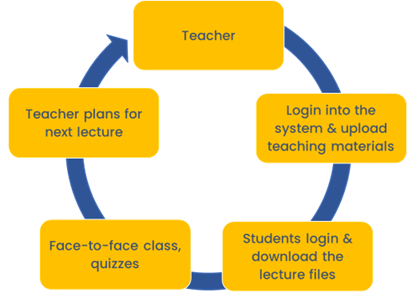
\includegraphics[scale=.9]{img/traditional.png}
    \caption{Traditional online enrollment system}
    \label{fig:System Architecture}
\end{figure}

The pandemic condition led to the transformation of formal education into online education with virtual classrooms that covered the fundamental needs for managing online education. IoT technology transforms classroom strategies in a useful way that makes it simpler to reduce time-consuming teacher and student practice concerns. In Bangladesh, though the online management system was maintained during the pandemic, after that it is being lost from the educational system. \\

As online education education is not practiced thoroughly in our country, results from online education are not always advantageous for the educational community since they raise a number of questions about the nature of online teaching and learning and raise public anxiety about the contentious subject of education. The current poll aims to illustrate the difficulties and opportunities faced by nations with less developed technology than those who have access to earlier contemporary technologies. \\

Despite not being in direct face-to-face contact with their instructors like in traditional classrooms, the majority of students have joined online classes with full enthusiasm, and informal surroundings have created a homely environment. However, internet disruptions and concerns about affordable bulk data availability remain significant challenges that need to be addressed to improve the education sector. It is essential to expand internet connectivity swiftly in distant locations and negotiate cost-effective data plans with cellular providers to assist students. These are the areas where national assistance is required to enhance the education system.\\

As the whole world and other universities of Bangladesh specially private universities are being virtualized, we also should build an online platform to keep pace with the modern world and to ensure effective and easier learning for the students.\\


\section{Problem Statement}
Under the current system, students are required to physically go and make appointments for final tasks without prior agreement on the subject with their teachers.
\begin{itemize}
    \item Under the current system, students are required to physically go and make appointments for final tasks without prior agreement on the subject with their teachers.

    
    \item Some researchers show that ongoing online platforms are not easier to access for sign-up.
    
    \item The results of the work can be beneficial to the governing bodies and owners of higher education institutions who are considering online education as a permanent fixture in the future.

    \item Some reliable systems are only available for the particular university and country.

    
    \item	Due to a shortage of resources, the online platforms in universities face numerous practical challenges.
    
    \item	There are many online platforms which can not provide not the security of data of the students and teachers. 

    
    \item Currently, either the main office staff or the lecturers themselves maintain the manual system, leading to an unnecessary increase in workload for the staff.

\end{itemize}


\section{Motivation}
In light of the decision of numerous knowledgeable students to pursue professional and academic opportunities at this university, it has expanded significantly over the years by adding new faculties and departments. However, this growth in enrollment has resulted in a declining relationship between professors and students throughout the university. Furthermore, the ratio of lecturers to students has decreased, making the current manual approach unsuitable for students who require guidance and wish to establish a better connection with their professors by meeting with supervisors.\\




\section{Objectives} 
This proposed system will serve the following objectives :
\begin{itemize}
    \item	To propose a novel model accompanied by easier methods, designed to function as a leading indicator and reduced complexity and time-consuming.


    \item	To develop this system by applying different user interfaces and also establishing a system according to the demands.

    \item	The proposed system will include detailed plans for hardware, operating systems, programming, and security considerations and  ensure the security issues for the users when they enter all of their personal data and information.



    % \item	The updated approach will try to address the shortcomings of the previous one while taking into account everyone from the supervisors to the pupils.


    % \item	The proposed system will include detailed plans for hardware, operating systems, programming, and security considerations.


    % \item	To ensure the security issues for the users when they enter all of their personal data and information.
\end{itemize}

% \newpage
\section{Research Outline}
The system is divided into four sections with different sub-sections and also demonstrated the required figures into it. In chapter II, there will be discussed related works in this area and which and how the model was used in those studies with detailed explanation. After that, I have briefed  the system model with the required figures to better understand in chapter III. For applying the models and building the system there will be needed the environment setup for programming and also the brief requirement analysis for this project which are entailed in the chapter IV. Then the implementation of the project will be shown and the result after applying different techniques are briefly explained in chapter IV. Finally, Chapter V will conclude the project by discussing potential areas for future work and improvements.








 \label{chap1:Literature}
 \chapter{Literature Review}

\section{Overview}
This chapter provides an in-depth review of the existing literature on student evaluation systems. It aims to explore various aspects of student evaluation systems, including their purpose, methodologies, effectiveness, and potential challenges. The literature review will serve as a foundation for understanding the current state of research and identifying gaps that need to be addressed in the subsequent chapters. Also the limitations of existing works have been shown in a table for better understanding.


\section{Review of Relevant Works}

The decisions of students to not pursue further education may have been influenced by a lack of direction in the supervision structure and shortcomings of their supervisors, resulting in reduced interaction with students. However, this issue could be effectively addressed by adopting online supervision.

Both students and teachers have worked hard during these terrible times, according to studies (as well as anecdotal data), and they still appreciate a sense of community and belonging, according to anecdotal evidence. Although technology has made it easier for staff and students to communicate with one another, it cannot take the place of a teacher. Both still prefer face-to-face instruction over the virtual or remote methods used to meet the pedagogical needs of students during the pandemic because face-to-face instruction offers intimacy that cannot be replaced by technology and digital tools are only meant to supplement face-to-face learning.\cite{sia2020facing}\\

Crossouard et al. found that changes in higher education courses have affected how teachers and students communicate using computers, and they advocate for supervisors to also adopt online supervision. This involves interpreting vocal and textual communication in the context of online supervision using computers.\cite{crossouard2008developing}

These findings support the study conducted by Hamzah et al. which showed that online supervision is an efficient method for students and supervisors to exchange knowledge, information, and track progress. Online supervision provides flexibility in terms of location and can be conducted under various conditions, as long as there is internet access, allowing both students and supervisors to choose the setting and location that suits them best.\cite{hamzah2017web}\\

Higher education students typically struggle to finish their research project within the allotted time.\cite{costa2018systematic} When it comes to students who are taking DL courses, this issue gets worse. Supervisors are essential to the process of research supervision, regardless of the type of schooling (DL or conventional). It's crucial that supervisors are motivated to watch over the kids. Workload agreements, time constraints, the caliber of the students, and acknowledgment of the supervisors' participation are four elements that have an impact on research supervisors.\cite{askew2016facilitators}\\


The appropriate and efficient use of ICT can create a supportive environment for both thesis students and supervisors. A study found that there was no significant difference between face-to-face and online tutoring using ICT. The use of ICT can be beneficial in providing frequent feedback and fostering a high level of interaction between students and supervisors.\cite{iwasaki2019design} \cite{hansen2015optimizing}\\

The paper titled "Supervision system of English online teaching based on machine learning" presents a comprehensive study on the implementation of an automated supervision system for online English teaching. The article emphasized the necessity for further exploration of the use of automated supervision techniques in high school education, and presented a new approach that combines remote supervision with machine learning algorithms (IRS-MLA).\\ Wen Lu, G. N. et al. explained how IRS-MLA mimics the implementation of supervision methodologies in the online English teaching process, based on actual requirements. The suggested approach entails evaluating the effectiveness of the teaching process by measuring students' performance and learning progress from both the teachers' and their students' perspectives. The paper does not provide a detailed discussion of the limitations of the proposed IRS-MLA system. It would be helpful to identify potential challenges and limitations that may arise in implementing the system in real-world settings. Additionally, the study focused on English language online teaching, and it remains unclear how the proposed approach may apply to other subject areas or disciplines. The paper could also benefit from a discussion of ethical considerations that arise when implementing an automated supervision system in online education, such as issues of privacy and data protection. Finally, while the study reports high levels of accuracy, efficiency, and success ratio compared to existing models, it would be useful to understand the degree of improvement over existing approaches and how the proposed system performs under different conditions and scenarios.\cite{lu2022supervision}\\

The role of Machine learning in Lockdown Exam Management Systems is comprehensively reviewed in the article. Sanaa Kaddoura, Daniela Elena Popescu, and Jude D. and their team effectively illustrate how the COVID-19 pandemic impacted the education sector, leading to the integration of Machine learning in the transition from traditional classroom-based learning to online learning and examination management systems. The article provides a systematic evaluation of 135 studies over the past five years, offering a well-rounded perspective on the various aspects of the exam cycle influenced by Machine learning. The authors categorize the unsupervised or supervised Machine learning algorithms in each process, highlighting their relevance and contribution to exam preparation, conduction, and evaluation. A notable strength of the article is the detailed examination of primary exam aspects such as authentication, scheduling, proctoring, and cheat or fraud detection from a Machine learning perspective. The authors' analysis of main attributes, including the prediction of at-risk students, adaptive learning, and student monitoring, enriches the understanding of Machine learning's role in exam preparation and management.\\
While the article presents a comprehensive overview of the role of Machine learning in Lockdown Exam Management Systems, it is essential to note some limitations. Firstly, the article mainly focuses on the use of Machine learning in the online examination system during the COVID-19 pandemic. The study does not cover the traditional classroom-based examination systems or the long-term impact of Machine learning on the education sector. Secondly, the article mainly discusses the technical aspects of Machine learning, such as authentication, scheduling, proctoring, and cheat or fraud detection, and does not delve into the ethical or social implications of relying heavily on technology for exam management. The study also does not provide insights into the students' perspectives on the use of Machine learning in the exam cycle. Thirdly, the article is limited to the available literature over the last five years. The fast-paced nature of technology may have led to new developments that are not covered in the study. Finally, while the article suggests solutions to the challenges and issues that Machine learning poses to the examination system, the implementation of these solutions may not be feasible or practical in all educational settings.\cite{kaddoura2022systematic}\\

I. Han, Wo. S. Shin et al. investigated the factors influencing the adoption of mobile learning management systems (LMSs) and the effects on students' academic achievement in higher education. The study collected data from 1604 students from an online university in Korea, including demographic backgrounds, psychological data, and external factors. The results showed that age and employment status significantly influenced the adoption of mobile LMSs, and there were potential connections between mobile LMS use and students' gender, age, and psychological characteristics. Furthermore, the use of a mobile LMS had a positive impact on online students' academic achievement. The study's large sample size allowed for generalizability of the results, and the use of logistic regression analysis provided a deeper understanding of the relationships among the variables studied.\\

However, the study has some limitations that should be considered. Firstly, the data was collected from a single online university in Korea, limiting the generalizability of the findings to other contexts. Secondly, the study's use of self-reported data may introduce response bias, as respondents may not always be truthful in their responses.\cite{han2016use} \\

In their study, Y. Fadol, H. Aldamen, S. Saadullah et al. shed light on the effectiveness of different modes of delivery in a management course at a business school in the Middle East. The authors compared the performance and perception of 122 students across three different modes of delivery: traditional, online, and flipped. The study's findings revealed that both online and flipped modes outperformed the traditional mode, with the flipped mode showing the highest performance. Moreover, absenteeism was lower in the flipped mode compared to the traditional mode, indicating higher student engagement in this mode. The study also found that accessing online material improved performance in both online and flipped modes, and students who accessed online material missed fewer classes in the flipped mode. Furthermore, the majority of the students perceived the flipped mode as more beneficial than the traditional mode. The study's strength lies in its comparison of various delivery modes and its use of both quantitative and qualitative data to support the findings. This finding is particularly noteworthy as it suggests that students may prefer a more interactive and engaging learning experience that promotes self-directed learning. The study's implications are significant, as they suggest that educational institutions should consider adopting innovative teaching strategies that are better aligned with students' learning preferences. The findings also indicate that online and flipped modes may be more effective in promoting student engagement and academic performance.\\

% \newpage
However, there are some limitations to this study that need to be addressed. Firstly, the study was conducted at only one institution, and the results may not be generalizable to other institutions or settings. Furthermore, the study did not evaluate the long-term effects of the different modes of delivery on students' academic performance. Nevertheless, the study's findings have significant implications for the development of future educational programs and highlight areas for further research. \cite{fadol2018comparative}\\

The article presents the development and evaluation of a new automated assessment tool for online distributed programming called DSLab. The authors recognize the complexity and difficulty of creating an automated assessment tool and aim to fill this research gap by providing a tool that can enhance students' academic performance in a meaningful distributed learning environment. The study employs a quantitative analysis method to collect and analyze data regarding students' perceptions of using the DSLab tool. The results suggest that the DSLab tool has acceptable utility and efficiency features and provides a valuable experience for students. The article's strength lies in its evaluation of the tool in a real, long-term online educational experience, adding to the validity of the findings. Additionally, the study identifies factors that can enhance the tool's design efficiency by suggesting new functionalities and ideas. However, the study is limited to a single case, and the generalizability of the findings may be constrained.\\

The article by T. Daradoumis et al. focuses on the creation and assessment of DSLab, an automated assessment tool for online distributed programming. While the study provides useful insights into the effectiveness and areas for improvement of the tool, there are some limitations that should be considered. The study only evaluates the tool's effectiveness from the students' perceptions, and the authors did not conduct any objective measurement of the tool's impact on students' academic performance. Thus, it remains unclear whether the use of the DSLab tool actually resulted in improved academic performance for the students. Again the study was conducted in a specific context, and the sample size was relatively small. Thus, it may not be possible to generalize the findings to other contexts or larger populations. Finally, the article does not discuss the potential drawbacks or limitations of using an automated assessment tool in online distributed programming. For example, some students may prefer more traditional forms of assessment or may feel uncomfortable with the technology involved.\cite{daradoumis2019analyzing}\\

The study conducted by I. Noguera, R. Masó et al. examines the effects of incorporating agile strategies into online collaborative learning, and its impact on engagement with learning activities and collaborative processes. Specifically, the research aims to determine if these strategies can enhance planning processes and regulate group work, leading to improved engagement. The study focuses on an undergraduate project-based learning course, and an iterative process of course redesign was conducted during two consecutive semesters. The new design was piloted and evaluated based on the students' and teacher's views and the learning outcomes. The research found that incorporating agile strategies was useful for improving students' online project management and collaboration. However, the study did not find any significant impact on students' satisfaction with the course or the overall learning outcomes. Despite this, the research provides valuable insights into the use of agile strategies for team regulation and project management in online higher education, which can help create a more effective learning environment.\\

One limitation of the study is that it focused on only one undergraduate project-based learning course. As a result, the findings may not be generalizable to other courses or educational levels. Additionally, the study did not measure the long-term impact of incorporating agile strategies on students' learning outcomes or their future collaborative experiences. It would be beneficial to conduct follow-up studies to determine if the strategies introduced in this study have a lasting impact on students' collaborative skills and experiences. Another limitation is that the study relied primarily on self-reported surveys and interviews to collect data. This may lead to biases in responses or limitations in the accuracy of the data collected. The study could have benefitted from using multiple data collection methods, such as observations or assessments, to provide a more comprehensive understanding of the impact of agile strategies on students' collaborative learning experiences. \cite{noguera2018collaborative}\\

R. Dad, S. N. Pasha, M. Sallauddin et al. implies that only a limited number of tools possess the ability to assess essays based on their content, and a smaller subset still are utilizing natural language processing techniques. Natural language processing is a powerful technique that can analyze and understand human language. The use of natural language processing in automated assessment tools could potentially revolutionize the way we evaluate essays. This study highlights the importance of assessment in the education system and the increasing interest in using automatic tools to aid in the assessment process. While there have been significant advancements in automatic assessment tools for objective-type questions, there is still room for improvement in the assessment of essays. The integration of natural language processing methods could potentially solve this problem and provide more accurate and reliable assessments of student essays.\\

One of the limitations of automated essay assessment tools is their inability to fully capture the nuances and creativity of human language. While natural language processing techniques have improved significantly in recent years, it is still difficult for automated tools to fully understand and evaluate the meaning and context of a piece of writing. Additionally, automated assessment tools may not be able to recognize more subjective aspects of writing, such as the emotional impact of a piece or the tone and voice of the author. These qualities may be important in certain types of writing, such as creative writing or personal narratives. Another limitation is that automated assessment tools may not be able to provide the same level of feedback and guidance that a human instructor can provide. While these tools can provide a score or grade, they may not be able to offer the same level of personalized feedback and constructive criticism that a human instructor can provide to help students improve their writing skills. \cite{dadi2020overview}\\

A.Shehab, M. Faroun, M. Rashad presents an informative review on the problems associated with manual grading and the need for auto-grading systems in the educational community. It highlights the advantages of auto-grading systems such as cost, time, and effort-saving compared to manual grading. The study also focuses on the specific challenge of developing auto-grading systems for Arabic languages due to complexities in morphology, semantics, and syntax. The research conducted a comparison of different algorithms used in automatic grading systems for Arabic languages using string and corpus algorithms separately. The use of multiple similarity measures and the introduction of an Arabic dataset containing 210 students’ answers make the study more comprehensive. The results obtained indicate that automatic grading systems can provide an effective solution for article grading systems.\\

The article could have included a discussion on the limitations of auto-grading systems. While auto-grading systems have many advantages, they are not without limitations. For example, they may not be suitable for assessing certain types of assignments that require subjective evaluation or critical thinking. Also, auto-grading systems may not be able to detect plagiarism, which can be a significant issue in the educational context. Furthermore, the study only focused on comparing different algorithms for automatic grading systems for Arabic language articles. It did not discuss the applicability of these algorithms in other contexts or for other types of assignments. Therefore, the generalizability of the results to other languages or assignment types is unclear. \cite{shehab2018automatic}

The importance of high-quality online course websites in facilitating effective learning experiences for students cannot be overstated. In this paper, S. Chakkrit et al. present an extended version of an evaluation framework for online courses and Learning Management Systems (LMS) that aims to address the shortcomings identified through its application in various e-learning courses. One of the key enhancements of the new version of the evaluation framework is the inclusion of a web-based questionnaire in both Thai and English languages. This addition makes it more accessible and user-friendly for a broader range of users, facilitating easier evaluation of online courses and LMS. Additionally, the authors have incorporated an authorization process, ensuring that only authorized individuals can access and complete the questionnaire, thereby enhancing the integrity of the evaluation process. Another notable feature of the extended framework is the introduction of a role-based evaluation process. This acknowledges the diverse perspectives and needs of different stakeholders involved in the evaluation, such as instructors, students, and administrators. By considering the unique requirements and expectations of each role, the framework enables a more comprehensive assessment of the online courses and LMS from multiple viewpoints. 

The authors state that the extended framework will be incorporated into O-DEST; they do not provide information on the practical implementation challenges that may arise during the integration process. Implementing an evaluation framework in real-world settings often involves various logistical, technical, and organizational hurdles that may affect its successful adoption and usage. \cite{snae2008web}


\section{Limitations of the Existing Systems}
In-depth comments or nuanced responses from students may not be possible in online student evaluation systems. The chance for instructors to follow up with students or explain input may not be offered, which could restrict the usefulness of the feedback given and leave open the possibility of failing to address any concerns or queries from the students. Additionally, the majority of current systems and models do not come with auto-marking systems.
\begin{table}[H]
\centering
\caption{A tabular format of various approaches along with limitations\\}

\begin{tabular}{ p{.5cm} p{5.5cm} p{7.5cm} } 
\hline
Ref. & Approaches & Limitations \\
\hline
[4] & Quantitative research on questionnaire survey  & Only did the research but was not able to build the system  \\ 
\hline
[9] & Proposed an automated IRS-MLA supervision system & The system was applied only on English online teaching and there was no guidelines on how to apply it on other topics\\ 
\hline
[10] & Categorized the system by Machine Learning Algorithms for exam management & The implementation system can not provide the feasibility in all types of educational settings \\ 
\hline
[15] & Assessed essays by NLP process tools & The tools was not able to provide any scores \\ 
\hline
\cite{shehab2018automatic} & Established an auto-grading system & The system was built only on Arabic Language which is not acceptable for all other educational institutes.\\
\hline
\end{tabular}
\label{table2.1}
\end{table}


 \label{chap2:Requirement Analysis}
 \chapter{Requirement Analysis}

\section{Overview}
In this chapter, there will be a discussion about the requirements of the project. Requirement analysis is the process of identifying, analyzing, and documenting the needs and expectations of the stakeholders for a software system. It is the first and most crucial step in the software development life cycle, and it involves understanding the user’s requirements and the system’s objectives. In this project, we have used VS code for building the online system. Here we use different types of language such as; HTML, CSS, and JavaScript. We also use SQL for a database where we store all information such as teacher information, student information, questions, tasks etc.

\section{User Requirement}
Any system, including web-based systems, must take the needs of its users into consideration when being designed and developed. The needs, expectations, and preferences of the system's users must be determined and given top priority while developing a web-based student evaluation system. A web-based student evaluation system is often used primarily by students, teachers, and administrators. It is crucial to comprehend their needs in order to make sure the system fits them and offers a positive user experience. Here are some important things to remember for each user group.
\begin{figure}[H]
    \centering
    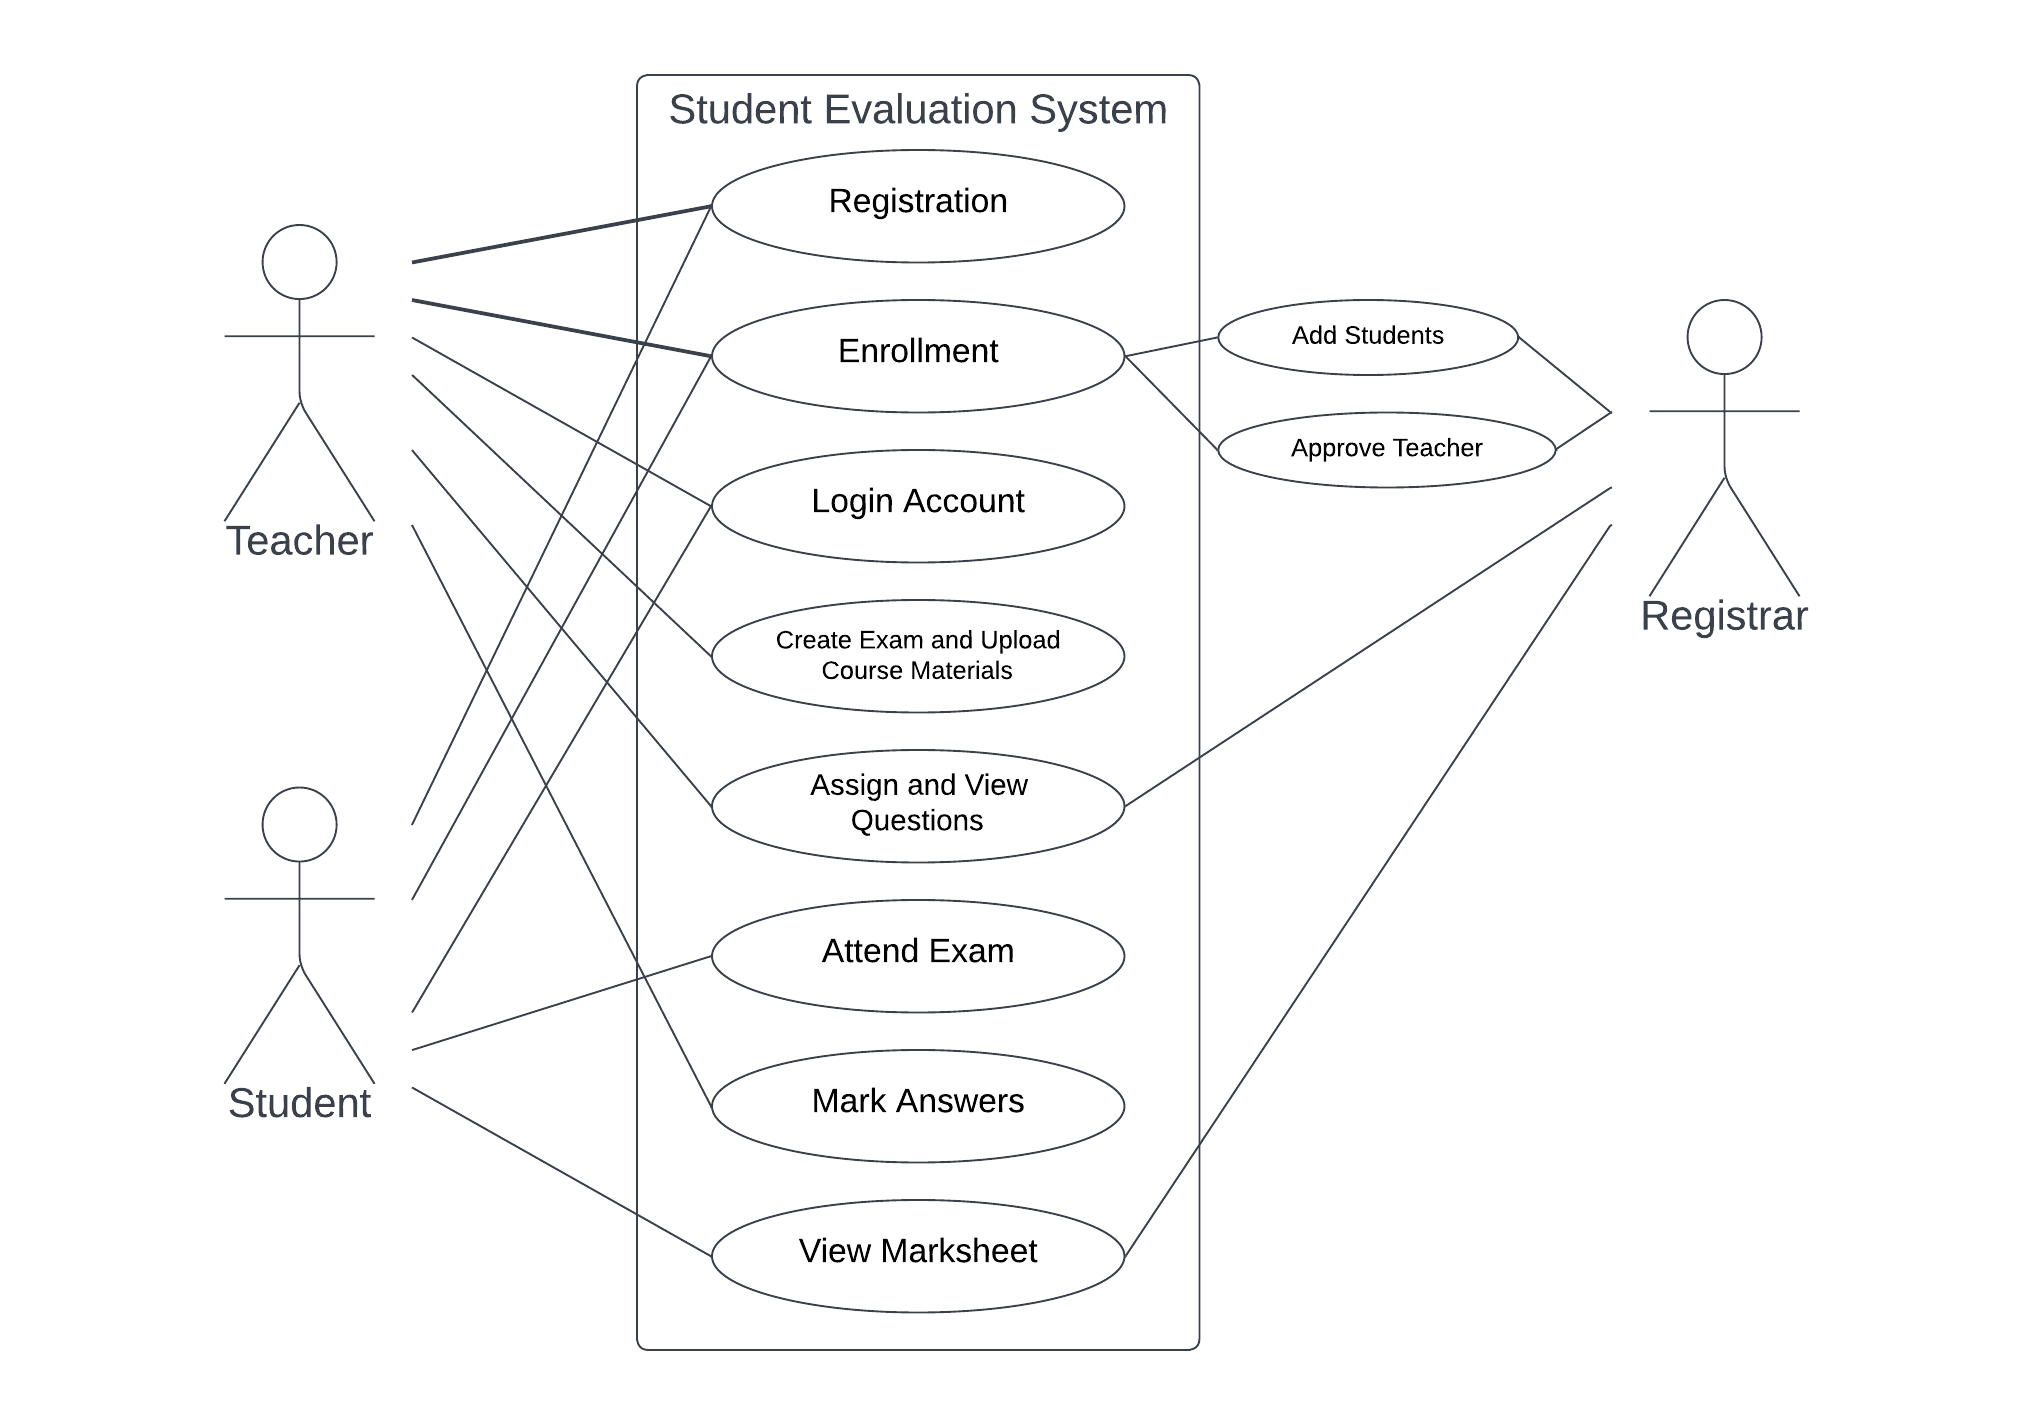
\includegraphics[scale=.2]{img/caseuml.png}
    \caption{Use Case Diagram}
    \label{fig:uml}
\end{figure}
A non-functional diagram provides an overview of the different aspects and characteristics of a system or process without detailing its internal workings. When it comes to online student evaluation, a non-functional diagram helps illustrate the non-functional requirements or qualities that the system should possess. The following figure of a non-functional diagram for an online student evaluation system illustrates the process to get registered as a user whether the user is a teacher or a student.\\

The functional diagram provides an overview of the system's major functions and their interdependencies. It helps stakeholders and system designers understand the flow of information and actions within the system, guiding the development and implementation process. 
Additionally, the functional diagram can serve as a basis for further decomposition into more detailed functional specifications for each component, ensuring a comprehensive and well-structured system design. 
\begin{figure}[H]
    \centering
    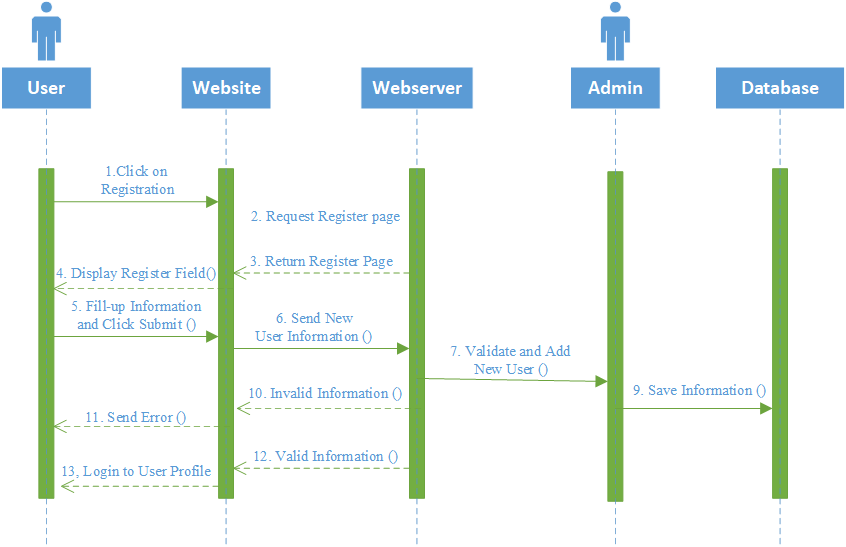
\includegraphics[scale=.7]{img/User.png}
    \caption{User Registration}
    \label{fig:uml1}
\end{figure}
In the case of an online student evaluation system, a functional diagram outlines the key functionalities and their relationships. The following figures show how a user can log in to the system and after being logged in what types of information the user will get.

\begin{figure}[H]
    \centering
    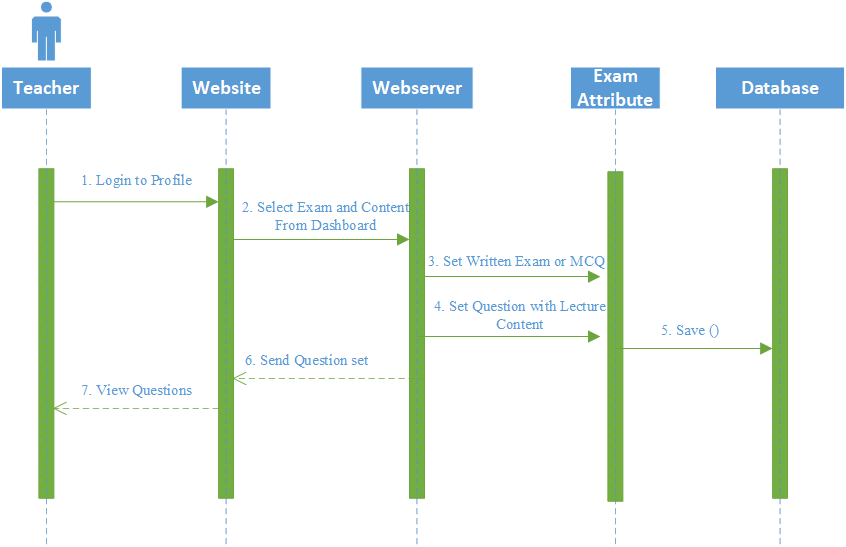
\includegraphics[scale=.7]{img/teacheruml.png}
    \caption{Teacher Set Question}
    \label{fig:uml2}
\end{figure}
From the above figure, we can see that a teacher will be able to create an exam and also there will be options to make both questions MCQ or written. The teacher will also be able to edit the questions if it is needed.
\begin{figure}[H]
    \centering
    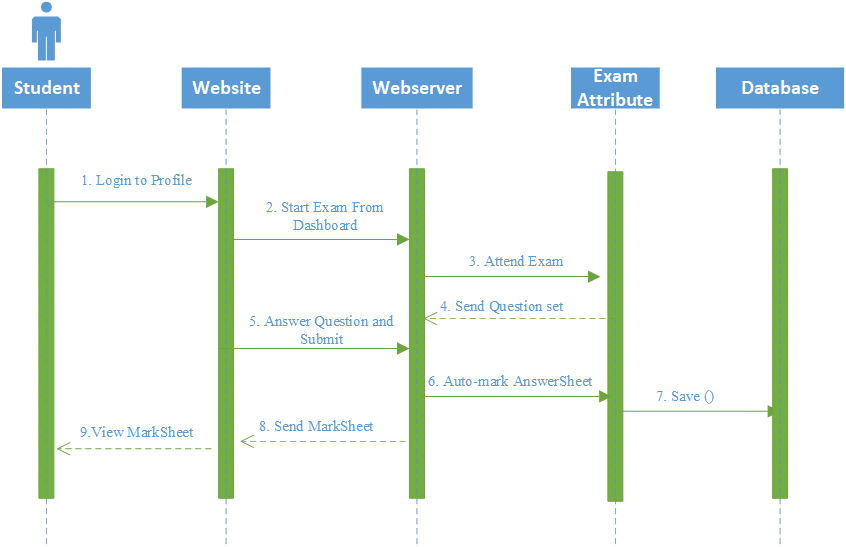
\includegraphics[scale=.7]{img/studentuml.png}
    \caption{Student Exam Attend}
    \label{fig:uml3}
\end{figure}
The above figure clearly shows that a student will be able to view the questions, attend the exams and submit the answer scripts. They will also be able to view the mark sheet of a particular exam from the website. 

\section{Software Requirement} 
This section explained software requirements, their importance, and their role in the development process. Software requirements serve as a foundation for designing, developing, and delivering successful software systems that meet the needs and expectations of users and stakeholders.

\subsection{VS code}
Visual Studio Code (VS Code) is a lightweight, cross-platform source code editor developed by Microsoft. It is free and open-source and supports a wide range of programming languages, making it a popular choice for developers worldwide. VS Code supports debugging for various programming languages, allowing developers to identify and fix bugs in their code. It has a vast library of extensions that provide additional functionality to the editor, making it more efficient and productive. VS Code comes with an integrated terminal that allows developers to run commands, scripts, and programs within the editor itself. The platform has built-in Git integration, enabling developers to manage source code repositories directly from the editor.
\subsection{Browser} 
Spider Browser is a modern and feature-rich web browser designed to provide users with a fast, secure, and customizable browsing experience. It offers a range of functionalities and tools that enhance productivity, privacy, and convenience while navigating the web.The customization options allow users to adapt the browser's appearance and functionality to their preferences, creating a personalized browsing experience. Spider Browser's optimized performance ensures fast and efficient browsing, enabling users to access web content quickly and smoothly.


\section{Language Requirement}
The section provides an overview of programming language requirements, their significance in software development, and their role in determining the choice of programming languages for different projects. Programming language requirements help define the specific programming languages that need to be used to develop software systems based on project needs and constraints.

\subsection{HTML}y
HTML (Hypertext Markup Language) is a markup language used to create and design web pages. It is the foundation of all web development and is used to structure and display content on the internet. HTML provides a set of elements or tags that define the structure and appearance of web pages. HTML is constantly evolving, with new versions introducing new features and improvements to existing ones. The latest version of HTML is HTML5, which includes new elements and features for multimedia, graphics, and interactive content.

\subsection{CSS} 
CSS (Cascading Style Sheets) is a stylesheet language used to describe the presentation and styling of HTML documents. It is used to control the layout, design, and visual appearance of web pages. CSS uses selectors to target specific elements in HTML and apply styles to them. Selectors can be based on element type, class, ID, attribute, and more. It provides a range of layout options, including grid, flexbox, and float. These layout options allow developers to create complex and responsive layouts for web pages. 

\subsection{JavaScript}
JavaScript (JS) is a high-level, dynamic, and interpreted programming language that is widely used to add interactivity and functionality to web pages. It is a client-side scripting language, meaning that it runs on the user's web browser rather than on a server. Javascript allows us to mark the mcq using local browser cookies of the examinee. It allows developers to write asynchronous code using callbacks, promises, and async/await, which enables the development of complex and efficient web applications.

\subsection{SQL} 
SQLite is a lightweight, open-source, and self-contained relational database management system (RDBMS) that is widely used in various software applications, including web and mobile apps. It is a serverless database, meaning that it does not require a separate server process to function and can be embedded directly into an application. SQLite is cross-platform and can be used on various operating systems, including Windows, macOS, Linux, and mobile operating systems like Android and iOS. 

\subsection{Django}
Django is a high-level, open-source Python web framework that is designed to help developers build complex, scalable, and maintainable web applications quickly and easily. It follows the Model-View-Controller (MVC) architectural pattern and emphasizes the "Don't Repeat Yourself" (DRY) principle, which aims to reduce code duplication and increase efficiency.
Django includes a powerful FORM that allows developers to work with databases using Python objects, rather than directly writing SQL code. It includes a powerful URL routing system that allows developers to map URLs to views, which are Python functions that handle HTTP requests. It also includes built-in security features, such as protection against SQL injection attacks and cross-site scripting (XSS) attacks.






 \label{chap3:SystemModel}
 \chapter{System Model}

\section{Overview}
The iterative enhancement approach is a software development methodology that involves building a system incrementally while incorporating lessons learned from previous iterations. The process entails starting with a basic implementation of software requirements and gradually improving the system through successive iterations. Each iteration involves adding new functional capabilities to the design. For the development of a website, it is essential to define the project requirements, create a backlog of tasks, and prioritize them based on importance and complexity. By adopting an Agile model, the developer can continually deliver new website features, ensure user satisfaction, and remain responsive to evolving requirements throughout the development process.\\
\begin{figure}[H]
    \centering
    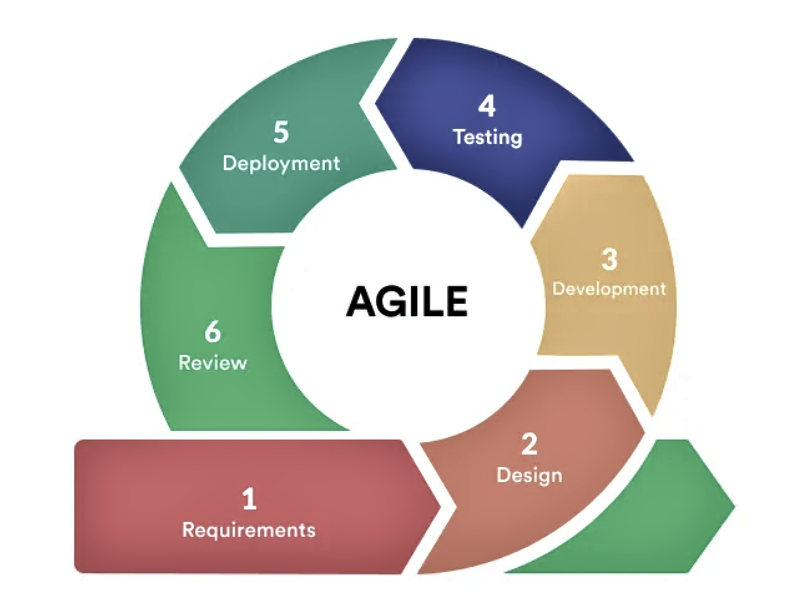
\includegraphics[scale=.6]{img/agile.png}
    \caption{The agile model}
    \label{fig:agile}
\end{figure}
The above model will help to build the web application step-by-step. This online system will help a university authority to follow up the department performance and it will be easier for both the users and admin panel. The students and the teachers will need to sign-up and login before enrolling in the system. The admin will check all the information provided by teachers and the students and also the admin will be responsible to give access to the account of them. For designing the process there have been used HTML, JavaScript and CSS and for the back-end and the database management Django and SQLite accordingly.\\


\section{Methodology}
Software performance guarantees that the application will function properly under a specific workload. The purpose of testing a system's performance is to confirm the responsiveness and functionality of particular features that were especially created for the system. Understanding how a software application behaves under a particular expected load and figuring out how resistant the application is under excessive stress are both crucial. Software performance demonstrates that the system satisfies the performance requirements. The system's burden or specific non-performing components can be found through performance testing. It is crucial for a new system's cost performance that attempts to create performance tests start as soon as the project is developed and continue as it moves forward. To understand better from both the teacher and student perspective here a picture is attached for understanding the whole process of this project.
\begin{figure}[H]
    \centering
    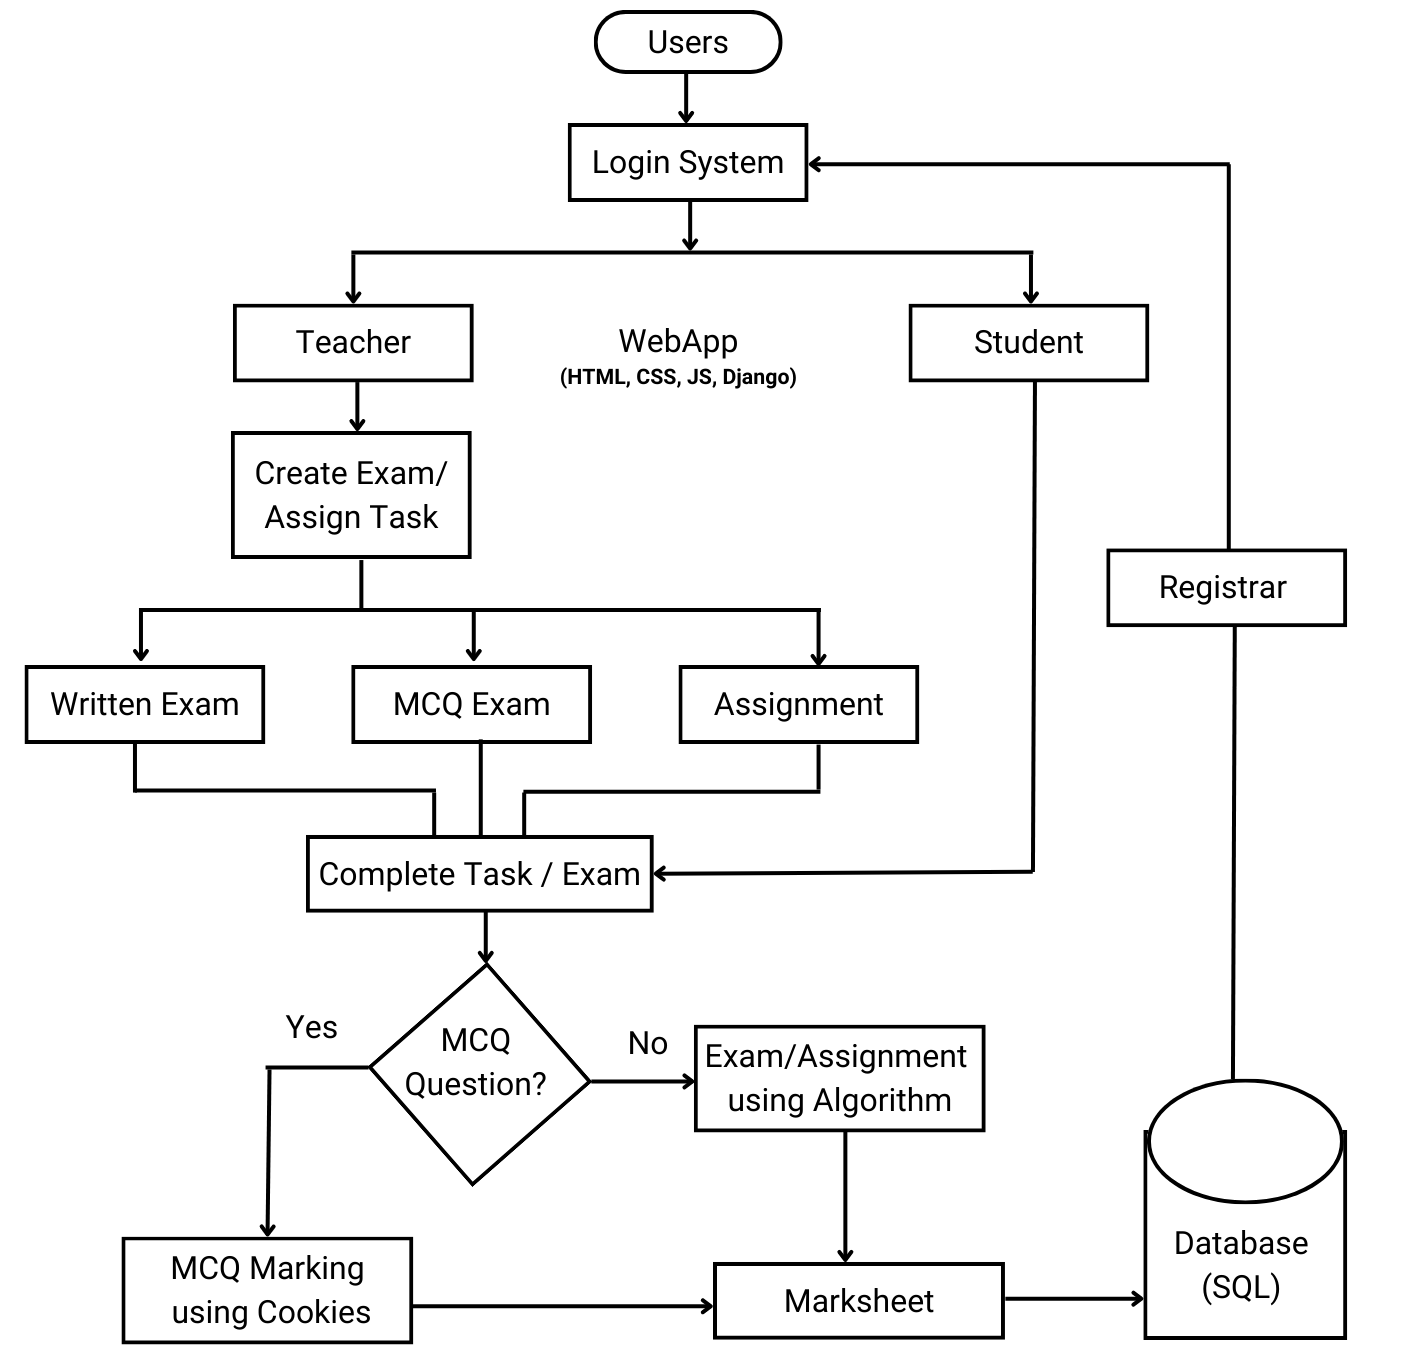
\includegraphics[scale=.36]{img/system-diagram.png}
    \caption{System Model}
    \label{fig:System}
\end{figure}
From the above figure \ref{fig:System} we can clearly understand that there will be two users to login into the system. The teacher will assign any kind of task which can be a mcq and written exam, assignment to the student and within a given period of time students will have to submit the task. MCQ exam will be evaluated or marked by the cookies of their local browsers and written exam or assignment will be evaluated by following machine learning algorithms. Then the assigned teacher will submit the marksheets of the students after evaluating. Finally the marksheet will be checked by the admin panel that means the registrar will check the final mark sheets from the database. \\

\section{System Design}
The system would require user authentication to ensure that only registered users, i.e. teachers and students, can access the system. A login page would be provided to the users, where they can enter their credentials to access the system. The system would have two types of users, teachers and students, each with their own set of permissions. Teachers would be able to create and assign tasks, evaluate submissions, and submit marksheets. Students would be able to view and attempt the assigned tasks, and submit their solutions. After evaluating the submissions, the teacher would be able to submit the marksheets of the students. The mark sheets would be stored in a database for further review. The admin panel, i.e. the registrar, would be able to access the database to review the final marksheets. The system would require a database to store the user information, tasks, submissions, and marksheets. The database would be managed using a database management system SQL. The system would be designed with security and privacy in mind. User data would be encrypted, and the system would use HTTPS for secure communication. User access would be restricted based on their roles and permissions, and regular backups would be taken to prevent data loss.

\subsection{Evaluation Process}
The online management system makes it possible to search and adds features like generating a task, approving the task, and letting the supervisor decide whether to accept the student or not. Both teachers and students' user profiles are kept up to date by the system administrator. The technology requires students to register an account before checking their credentials against faculty records. While it is necessary to take the class with the teacher, communication takes place by email. As it is said before, the evaluation process will be two types for evaluating the written types and mcq types.

\newpage
\subsubsection{Written Paper Mark Calculation}
The written ones will be checked for similarity by machine learning algorithms and marked accordingly. The process has been given below:\\

\begin{figure}[H]
    \centering
    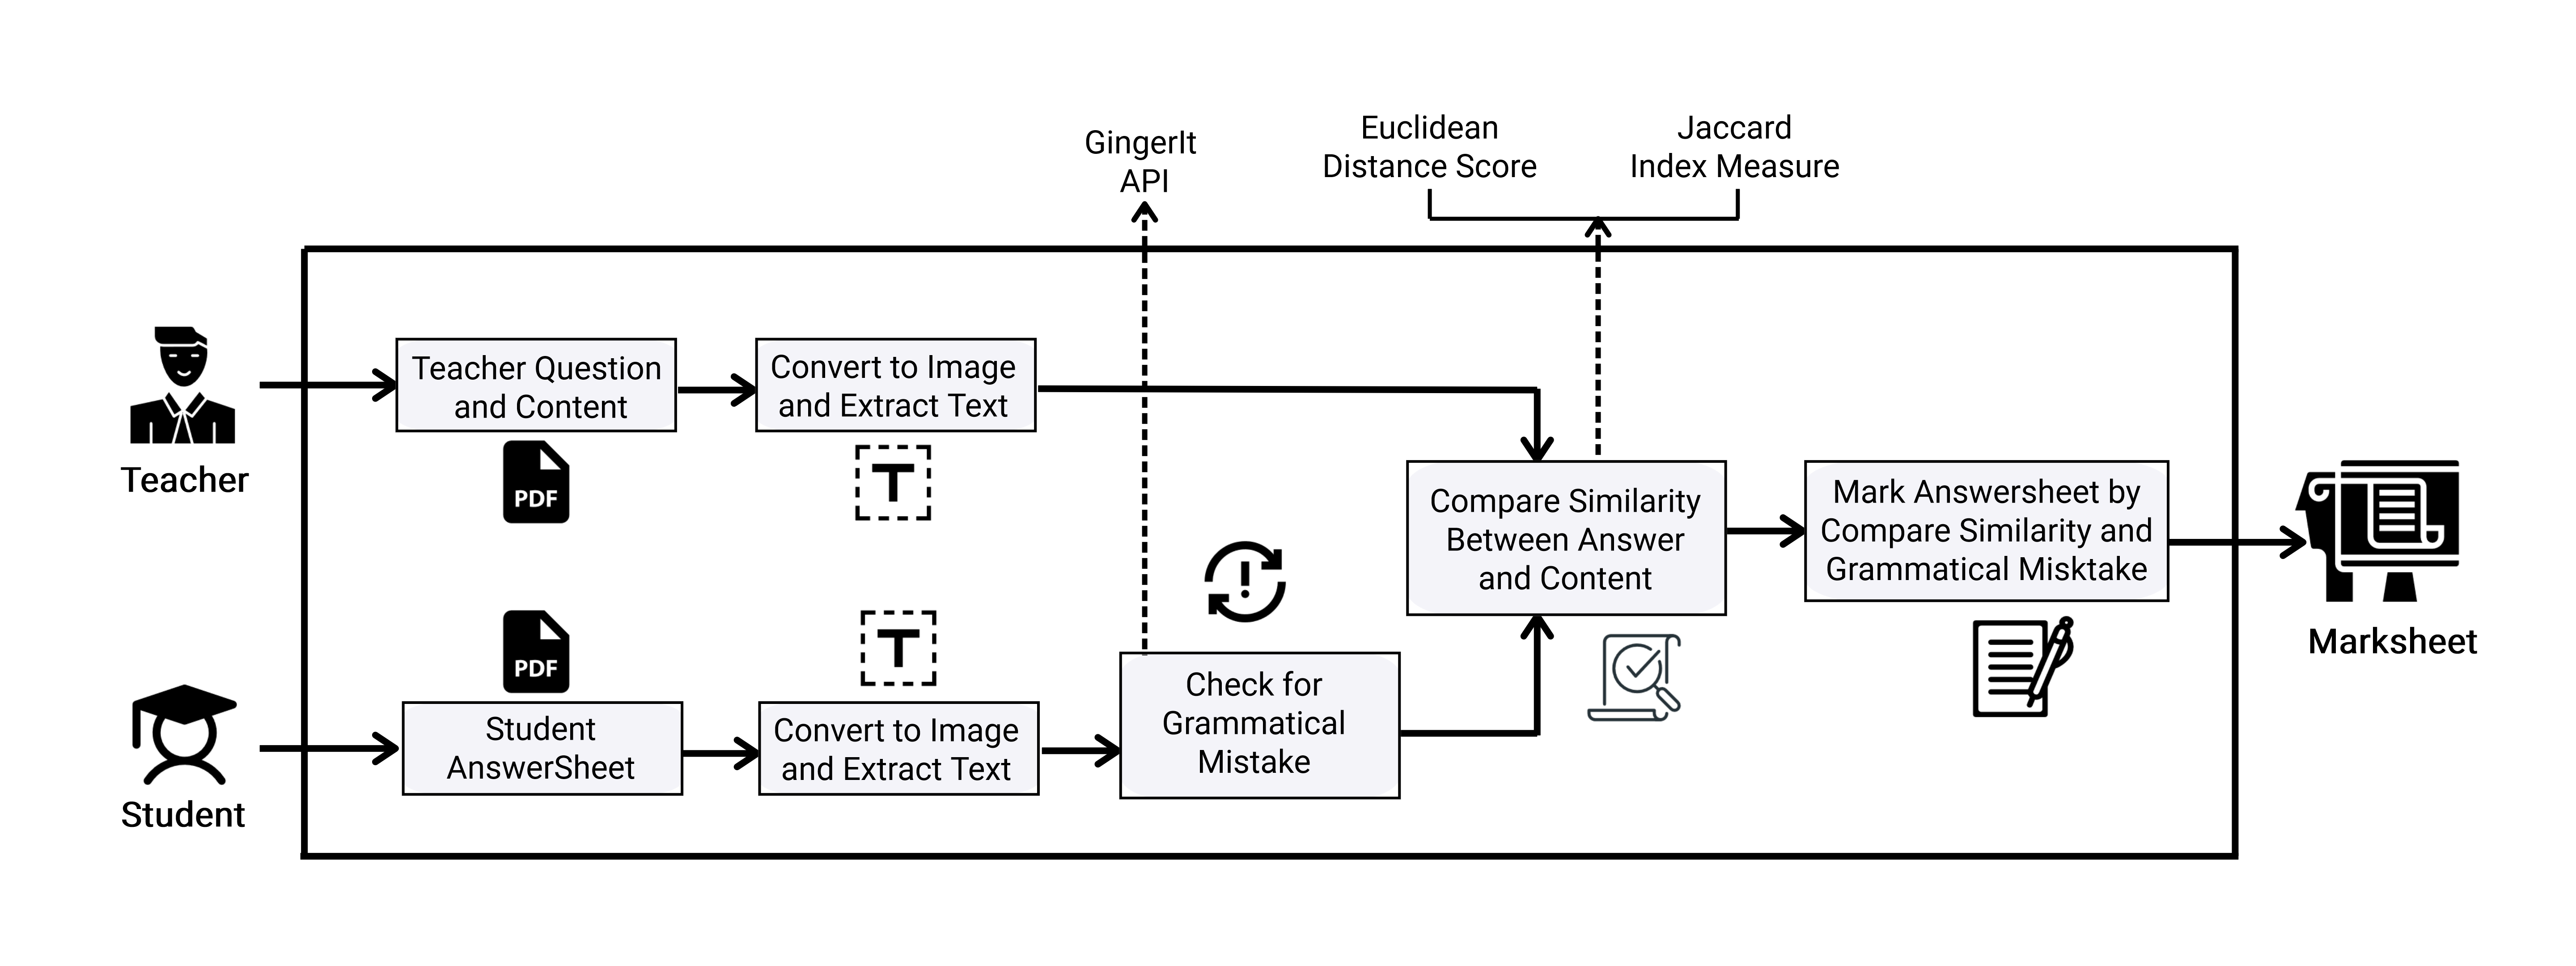
\includegraphics[scale=.07]{img/written.png}
    \caption{The written part evaluation process}
    \label{fig:written}
\end{figure}

In the above figure \ref{fig:written}it can be seen that after getting the answer sheet, the file will be converted into an image and we will need to extract the text. After that, the grammatical mistake will be checked and also the similarity will be checked by machine learning algorithms. In this project, it has been tried to use Euclidean Distance Score and Jaccard Index Measure for the similarity check. The two algorithms working flow is given below:
The very first algorithm which is used to find the similarity of the written task is Jaccard Index. It is also known as the Jaccard similarity coefficient, is a statistic used to measure the similarity between two sets of data. It is defined as the size of the intersection of the sets divided by the size of the union of the sets. Mathematically, the Jaccard distance can be expressed as:

$J\binom{A}{B} = \frac{ |A \cap B|} {|A \cup B|}$

where A and B are two sets, $|A|$ and $|B|$ represent their respective cardinalities (i.e., the number of elements in each set), and $\cap$ and $\cup$ denote the intersection and union of the sets, respectively. The Jaccard index ranges from 0 to 1, where a value of 0 indicates that the two sets have no common elements, and a value of 1 indicates that the sets are identical. The Jaccard index is commonly used in data science, information retrieval, and natural language processing to measure the similarity between two sets of words, documents, or other types of data.

\begin{algorithm}[H]
\caption{Jaccard Index Measure}\label{alg:Jaccard}
\begin{algorithmic}[1]
\State \textbf{Input}$ (set\_A, set\_B)$
\State $ set\_C \gets \emptyset $

\If{$set\_C \cap  set\_B$}
    \State $set\_C \gets set\_A \cap set\_B$
\EndIf

\State $set\_D \gets \emptyset $
\If{$set\_D \cup  set\_B$}
    \State $set\_D \gets set\_A \cup set\_B$
\EndIf  

\State $j\binom{A}{B} = \frac{set\_C - set\_D }{set\_D} $

\If{$j = 0 $}
    \State \textbf{Return}
\textit{True, $j\binom{A}{B}$}
\EndIf  
\\\textbf{Return}
\textit{0}
\end{algorithmic}
\end{algorithm}

The Euclidean Distance Score is a measure of similarity or dissimilarity between two vectors in a Euclidean space. It is calculated as the square root of the sum of the squared differences between the corresponding elements of the two vectors. Mathematically, it can be expressed as:

$d(\mathbf{a}, \mathbf{b}) = \sqrt{\sum_{i=1}^{n} (a_i - b_i)^2}$

where $\mathbf{a}$ and $\mathbf{b}$ are two n-dimensional vectors. The Euclidean Distance Score is commonly used in various machine learning and data mining algorithms, such as k-Nearest Neighbors, clustering, and dimensionality reduction. It is especially useful in cases where the features of the vectors represent physical measurements or geometric attributes.


\begin{algorithm}
\caption{Euclidean Distance Score}\label{alg:euclidean}
\begin{algorithmic}[1]

\Ensure Vectorize $N$ Dimention of $(set\_a, set\_b)$
\State $\textbf{Initialize} (distance_i = 0, sum\_square_i = 0)$

\For {$i$ in $N$}
    \State $difference_i = set\_a_i - set\_b_i$
    \State $sum\_square_i$ = $sum\_square_i + difference_i^2$
    
\EndFor
\State $distance_i = \sqrt{sum\_square_i}$

\\\textbf{Return}
\textit{$distance_i$}
\end{algorithmic}
\end{algorithm}


\newpage

\subsubsection{MCQ Mark Calculation}
Another algorithm \ref{alg:MCQ} shows the way that MCQ marking is being done during assessment of the student’s mark sheet. The input to the algorithm is a set of questions and their respective correct answers. The algorithm works by iterating through the questions in the set and checking if the answer given by the student matches the correct answer. If the answer is correct, the value of the corresponding cookie is added to a cookie set. After checking all the answers, the algorithm then iterates through the cookie set and compares the values to the correct answers. For each match, the total mark is incremented by 1. Finally, the total mark is returned as the output of the algorithm.


\begin{algorithm}
\caption{MCQ Marking}\label{alg:MCQ}
\begin{algorithmic}[1]
\State \textbf{Input}$ (questions\_set, questions\_answer)$

\For{$questions \in questions\_set$}
    \If{$check\_answer$}
        \State $cookies\_set$ \textbf{add} $check\_answer.value$
    \EndIf
\EndFor

\State $ total\_mark = 0 $
\For{$value \in cookies\_set$}
    \If{$value = questions\_answer$}
        \State $total\_mark$ \textbf{=} $total\_mark$ + 1
    \EndIf
\EndFor

\\\textbf{Return}
\textit{total\_mark}
\end{algorithmic}
\end{algorithm}



 
 \label{chap4:Implementation}
 \input{chapters/chapter5}

 \label{chap5:Conclusion}
 \chapter{Conclusion and Future scope}

\section{Overview}
This chapter serves as the conclusion of the research study on student evaluation systems. It synthesizes the findings from the empirical research conducted and presents a comprehensive summary of the key insights gained. Additionally, this chapter identifies potential areas for future research and suggests recommendations for improving student evaluation systems.

\section{Conclusion}
In conclusion, the creation and implementation of a web-based system for student evaluation has the potential to completely transform the way that educational institutions evaluate their students. Utilizing web-based platforms has many benefits, including efficiency, accessibility, and ease. Educational institutions can improve data management, simplify administration, and streamline the evaluation process by switching from conventional paper-based evaluation methods to a web-based approach. Students can conveniently offer their input through the evaluation system using online browsers, which eliminates the need to physically collect and handle evaluation forms.

% \newpage
\section{Future Scopes}
Online student evaluation systems have already gained widespread popularity due to their convenience and efficiency. As technology continues to advance, the future scope of online student evaluation systems is likely to expand further. Here are some potential future developments:

\begin{itemize}
    \item	Online student evaluation systems can leverage data analytics and machine learning to provide personalized feedback and learning paths to students. In the future, these systems could become even more intelligent, offering students personalized content and assessment that is tailored to their individual needs and abilities.

    \item	As online education continues to gain traction, it is likely that online student evaluation systems will become more integrated with learning management systems. This would allow for more seamless tracking of student progress and performance, and could provide instructors with greater insights into how to tailor their teaching strategies to better meet student needs.

    \item	Gamification is a technique used to engage learners and motivate them to learn by incorporating game elements into the learning experience. Online student evaluation systems can potentially adopt gamification techniques to make the evaluation process more engaging and motivating for students.

    \item	As more and more sensitive information is collected through online student evaluation systems, it is essential that these systems have robust security measures in place. In the future, online student evaluation systems are likely to become even more secure, with features such as two-factor authentication and encryption becoming more prevalent.

    \item	Online student evaluation systems can provide students with immediate feedback on their performance. In the future, these systems could incorporate advanced feedback mechanisms, such as the use of natural language processing (NLP) to provide more detailed and actionable feedback to students. This could help students to identify specific areas of strength and weakness, and to make targeted improvements in their learning.

    \item	The platform will be used to take live video classes for more engagement of the students. For which other video calls apps won’t be needed to take classes. In one platform the teachers and students will find their facilities.
\end{itemize}

\label{chap4:Reference}
\bibliographystyle{ieeetr}
% \renewcommand{\bibname}{Bibliography}
\bibliography{ref.bib}

\end{document}
